\section{Results}

\subsection{Theoretical Hit Rate Analysis}
blabla we want to know what the scaling of speedup looks like when we arbitrarily simulate a cache hitrate for some algorithms. This does not take into account cost of eviction and caching. 

We find that in most cases caching can significantly improve query execution time, with improvements scaling predictably as hit rate increases. 
For some long-running queries such as interactive-discover-6, 7, and short-3 no speedup is observed, with some queries even showing slower result production. 
These query templates traverse many solid pods, but do not require all traversed data. 
In such cases, we hypothesize that having access to a cache which serves documents from memory will quickly produce too much data and slow down result production. 
Thus, waiting for HTTP responses between traversal steps allows the JavaScript event loop to run the join execution pipeline and thus produces results faster as only the first few requests are required for first results.
\begin{figure*}[!h]
    \centering
    % Ensure the filename matches your generated PDF
    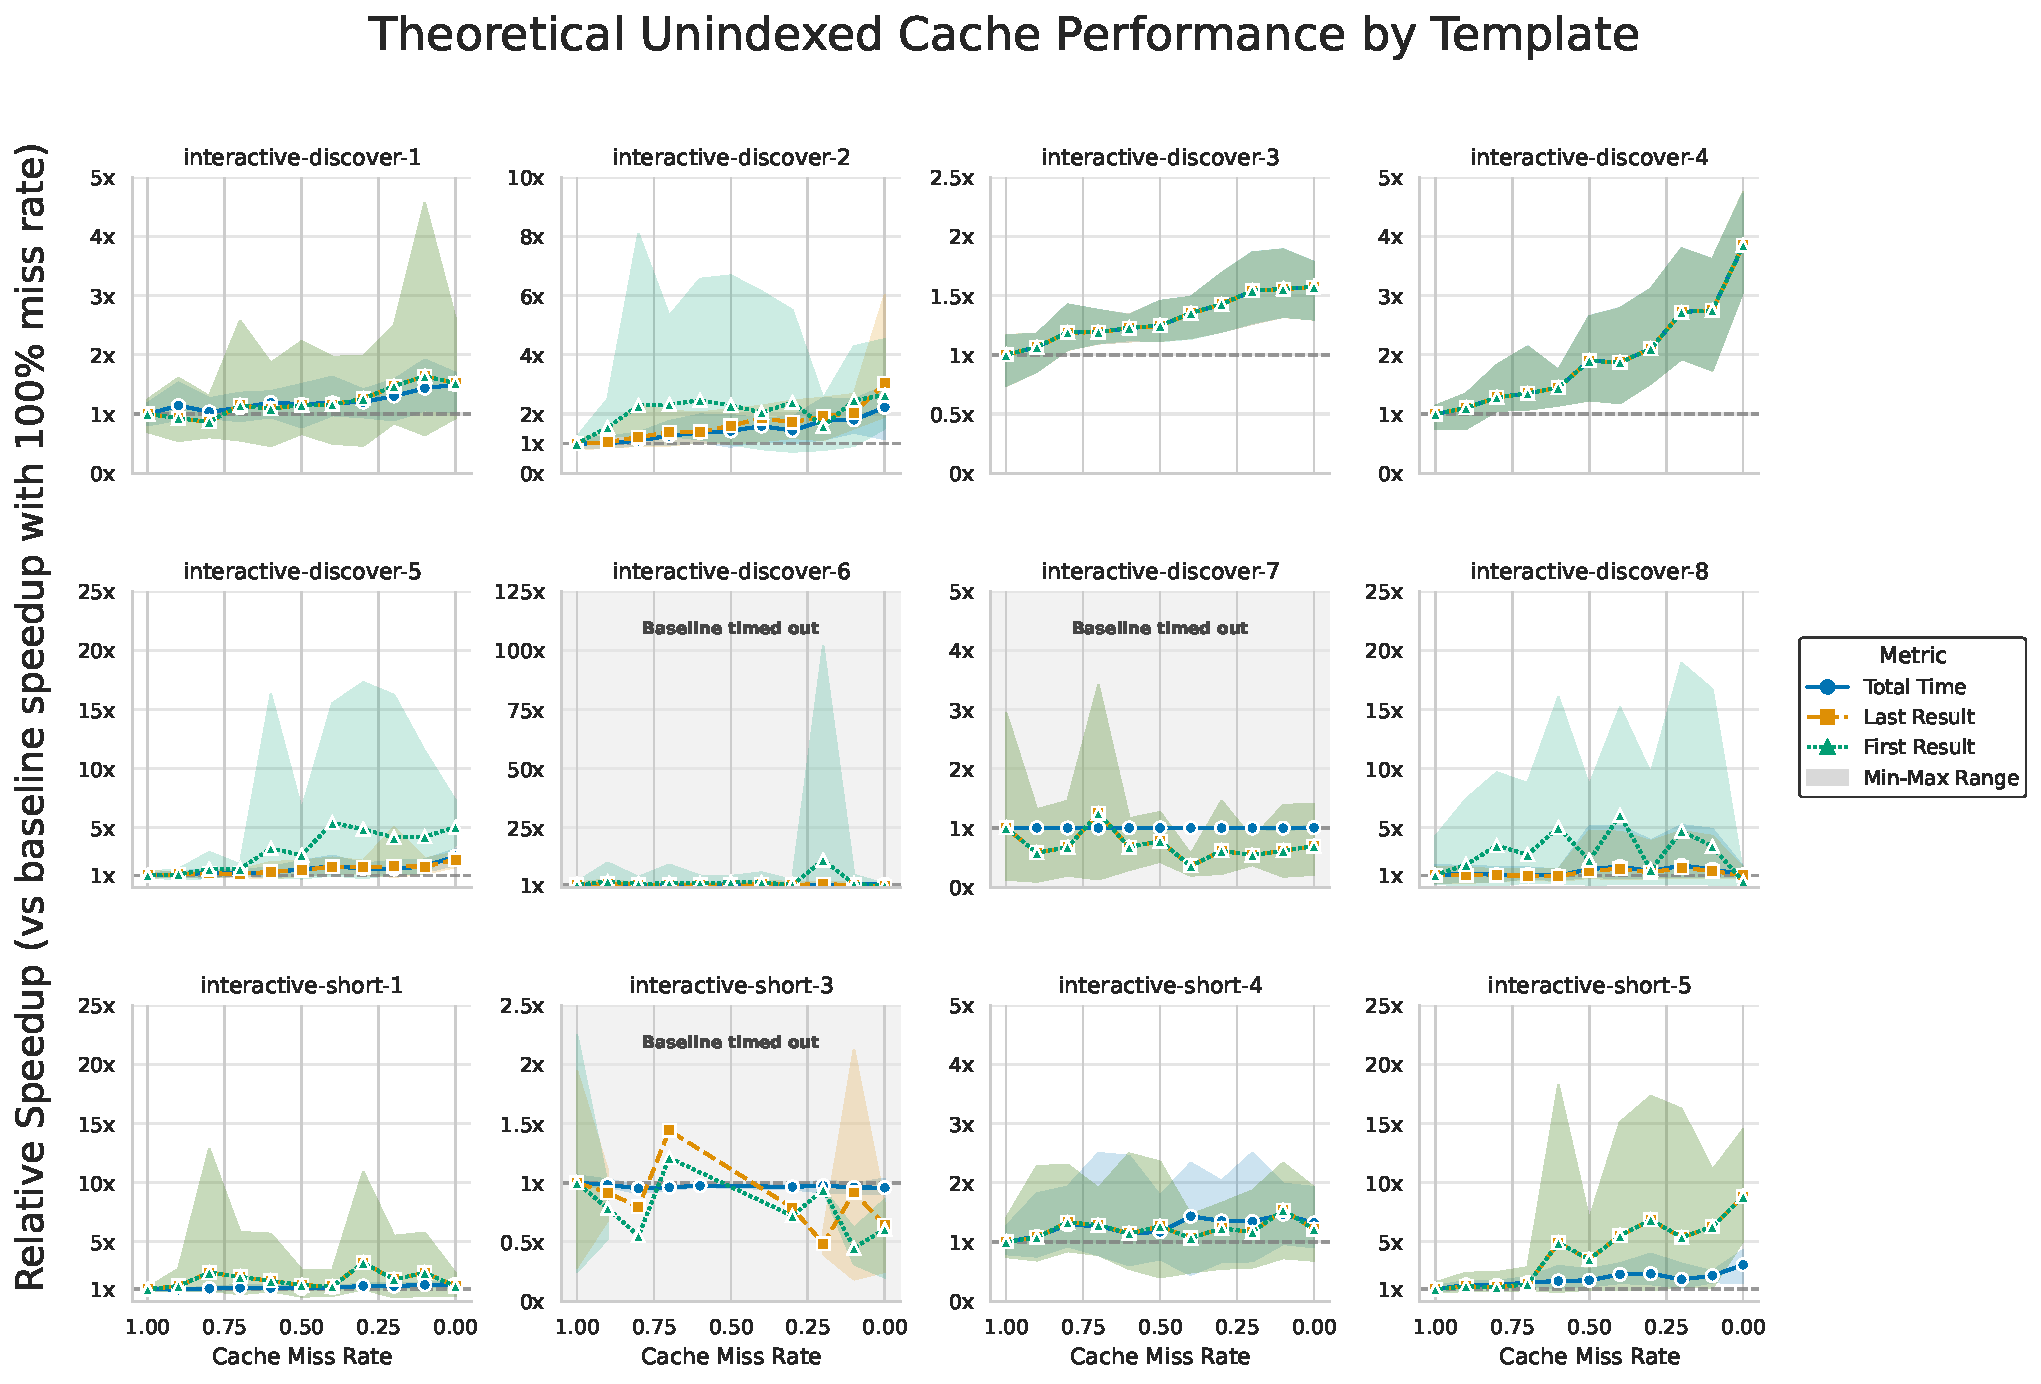
\includegraphics[width=\textwidth]{figures/cache_performance_trellis_academic.pdf}
    \caption{Theoretical unindexed cache performance by query template. Lines indicate the mean relative speedup of the repeated query for total execution time, first result, and last result against a $100\%$ miss rate baseline. Shaded regions denote the absolute minimum and maximum variance across iterations.}
    \label{fig:theoretical_cache_performance}
\end{figure*}